% 15/11/2020 - First round of corrections: added Thomas (new) & Ray corrections
% 15/11/2020 - Grammarly

\begin{refsection}
\chapter{Correcting optical imperfections in refractive lenses}\label{sec:corrections}

The interest and possibility of arbitrarily manipulating the X-ray wavefront has been teased since, at least, the early 2000s [\cite{Chubar1999, Chubar2001b}]. It was not until the advent of extremely accurate additive and subtractive manufacturing techniques [\cite{Stohr2015, Polikarpov2016, Petrov2017, Roth2018, Sanli2018, Seiboth2019, Abrashitova2020, Antipov2020, Lin2020, Medvedskaya2020}] that the demonstration of free-form X-ray refractive optics was done [\cite{Sawhney2016,Seiboth2017,Laundy2019, Seiboth2020, Dhamgaye2020}]. The possibility of producing very accurate free-form optics for the correction of optical aberrations has brought renewed interest in wavefront sensing [\cite{Berujon2015, Seaberg2019}] and optical design simulations [\cite{Laundy2020}]. This chapter presents the early results on correcting optical imperfections in refractive lenses obtained at the ESRF. The design and expected performance is based on the lenses presented in \S\ref{sec:single_lens}~-~\textit{\nameref{sec:single_lens}} and the simulations shown in Chapter~\ref{sec:effect_optical_imperfections}~-~\textit{\nameref{sec:effect_optical_imperfections}}.

%-------------------------------------------------------------------------
%-------------------------------------------------------------------------
\section{Corrective optics}\label{sec:corrective_optics}
%-------------------------------------------------------------------------
%-------------------------------------------------------------------------

Correcting optical imperfections can be done by actively reshaping an optical element (adaptive optics) [\cite{Sutter2012, Alcock2013}] or by inserting a static (passive) optical element specially fitted to compensate the deviations from a perfect profile or the wavefront error in relation to an idealised intensity [\cite{Donato2020}] or phase profile. Phase manipulation for wavefront manipulation can be done with diffractive elements [\cite{Probst2020}] or with refractive elements [\cite{Sawhney2016,Seiboth2017,Laundy2019,Seiboth2020, Dhamgaye2020}]. As indicated by the vast literature, refractive optics is the most popular method for correcting phase errors in partially-coherent X-ray beams. This section presents the design of refractive optical correctors for refractive lens stacks.

%-------------------------------------------------------------------------
%-------------------------------------------------------------------------
\subsection{Design}\label{sec:design}
%-------------------------------------------------------------------------
%-------------------------------------------------------------------------
\begin{figure}[t]
        \centering
        {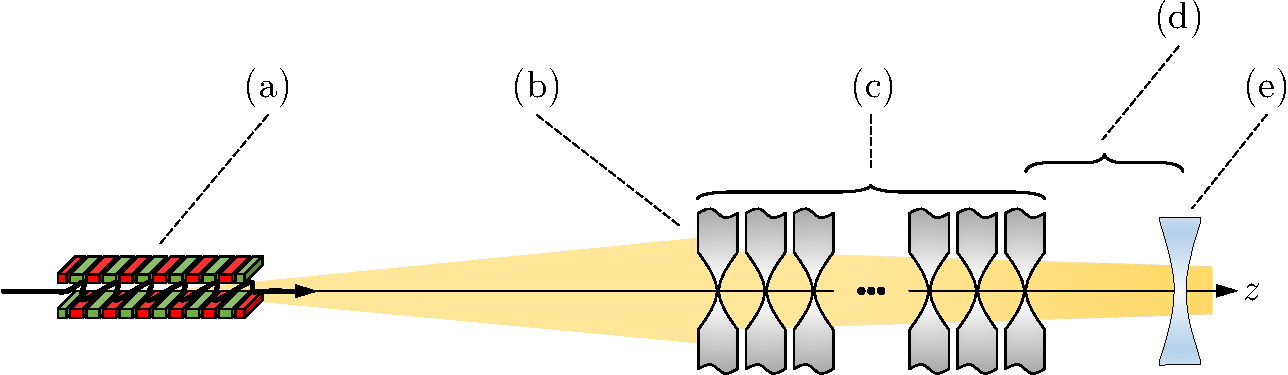
\includegraphics[width=0.6\linewidth]{figures/ch06/phase_extraction.pdf}}
        \caption[Schematic for phase correction calculation]{Schematic for residual phase extraction. (a) an arbitrary X-ray source delivers a (b) wave-field $U_{\text{illum.}}(x,y)$ immediately before the (c) optical system being studied. The wave-field exits the optical system and can be propagated a (d) distance $\Delta_{z_\text{pp}}$ from the exit pupil. At this position, the (e) extraction of the ideal phase from $U_{\text{exit}}(x,y)$ is done according to Eq.~\ref{eq:phase_corr}.}\label{fig:phase_extraction}
\end{figure}
Formally, the computation of the phase correction\footnote{The design of optical correctors for synchrotron radiation was first described in [\cite[\textit{§2}]{Chubar1999}], revisited in [\cite{Chubar2001b}] and first implemented for a 2D CRL in [\cite{Seiboth2017}].} for any optical system is done by assuming that the wave-field will develop a specific phase $\phi_{\text{exit}}(x,y)$ distribution after passing through an arbitrary optical system. Perfect focusing of a wave-field to a point-source at a distance $r$ from the exit pupil requires that the developed phase $\arg [U_{\text{exit}}(x,y)]$ to be that of a spherical-wave as in Eq.~\ref{eq:spherical} [\cite{Chubar1999}]. Given the typical geometric apertures and focal distances of a CRL composed of a few individual lenses\footnote{Assuming that the focusing inside the CRL is negligible - cf. [\cite{Schroer2005}] and [\cite[\textit{\S6}]{Seiboth2018}].}, it is possible to use the phase of the paraxial approximation of Eq.~\ref{eq:spherical}, that is, the parabolic-phase of the wavefront in Eq.~\ref{eq:parabolic}. If the wavefront illuminating the optical system is given by $U_{\text{illum.}}(x,y)$, then, after passing through an aberrated lens system, $U_{\text{exit}}(x,y)$ is given by:
\begin{equation}\label{eq:U_exit}
    U_{\text{exit}}(x,y) =   \mathcal{D}(\Delta_{z_\text{pp}})\cdot\left[\mathrm{T}_{\text{CRL-MS}}(\Delta_z) \cdot U_{\text{illum.}}(x,y)\right],
\end{equation}
where $\mathcal{D}(\Delta_{z_\text{pp}})$ is a free-space propagation from the exit pupil of the optical system to the position along the optical axis where the phase correction is performed (Eq.~\ref{eq:Fresnel_operator}) and $\mathrm{T}_{\text{CRL-MS}}(\Delta_z)$ is the operator description of a lens stack given by Eq.~\ref{eq:TE_CRL_MS_ERR}. The phase shift necessary to correct such wavefront can be calculated as:
\begin{equation}\label{eq:phase_corr}
   \phi_{\text{correction}}(x,y) = \arg\left[\cfrac{\exp{\Big(-ik\frac{x^2 + y^2}{2z_f}\Big)}}{U_{\text{exit}}(x,y)}\right].
\end{equation}
Where $z_f$ is the distance from the phase corrector to the image plane [\cite{Seiboth2017}]. This phase extraction procedure is illustrated in Fig.~\ref{fig:phase_extraction}. A phase corrector based on refractive optics can be calculated directly from the phase obtained in Eq.~\ref{eq:phase_corr} and the transmission element in projection approximation phase-thickness relationship described by Eq.~\ref{eq:aux_funcs_transb}:
\begin{equation}\label{eq:phase_plate}
   \Delta_\text{pp}(x,y)=-\frac{\phi_{\text{correction}}(x,y)}{k\delta_\text{pp}(x,y)}.
\end{equation}
Where $\Delta_\text{pp}(x,y)$ is the local phase plate thickness in projection approximation and $\delta_\text{pp}$ is the refraction index decrement of the material used for correcting $ \phi_{\text{exit}}(x,y)$. The resulting correction plate described by Eq.~\ref{eq:phase_plate} is directly proportional to the phase errors at each $(x,y)$ coordinate pair. Typical error maps are shown in Figs.~\ref{fig:metrology_zernike_profiles}, \ref{fig:recovered_thickness}, \ref{fig:accumulated_profile_1}-\ref{fig:CDo}. Current micro- and nanofabrication techniques used for manufacturing X-ray optics\footnote{Current for micro- and nanofabrication of 3D structures include: } are capable of reproducing such intricate shapes with high spatial and depth resolution, however the use of such correction plate in an experimental setup is rather impractical due to the several degrees of freedom concerned when aligning it against the aberrated optical system. Furthermore, it has been observed that 2D lenses produced by (hot) embossing are dominated by spherical aberration terms (primary, secondary, tertiary...) and other azimuathally symmetric errors due to intrinsic manufacturing processes [\cite{Schropp2013, Uhlen2014, Seiboth2016, Seiboth2017, Celestre2020, Seiboth2020}] -  see also the Zernike polynomial bar plots (orange bars) in Figs.~\ref{fig:metrology_zernike_profiles}, \ref{fig:recovered_thickness}, \ref{fig:accumulated_profile_1}-\ref{fig:CDo}. Trading some of the correction accuracy for more practicality when employing the correction plate in a beamline, it is possible to obtain a correction profile by azimuthally averaging $\Delta_\text{pp}(x,y)$:
\begin{equation}\label{eq:phase_plate_r}
   \Delta_\text{pp}(r)=\cfrac{\displaystyle\int\limits_{0}^{2\pi}{\Delta_\text{pp}(r,\theta)r\text{d}\theta}}{\displaystyle\int\limits_{0}^{2\pi}{r\text{d}\theta}},
\end{equation}
where $r=\sqrt{x^2 + y^2}$ and $\theta=\arctan{\big(y/x\big)}$ are the transformation from Cartesian to polar coordinates. The correction plate as calculated by Eqs.~\ref{eq:phase_plate} and \ref{eq:phase_plate_r} is tailored for a specific set of lenses operating at a defined energy, due to the dispersion properties of $\delta_\text{pp}$. Although true that a correction plate design is suited to a specific lens combination, for a moderate number of lenses where the focusing inside the CRL can be neglected, it has been demonstrated that the correction plate can be used over a range of energies around the design energy $\text{E}_\text{design}$ as the index of refraction decrement $\delta$ is proportional to $\lambda^2$ [\cite[\textit{\S6}]{Seiboth2018}]. This can be done by shifting the plate along the optical axis closer or further away from the design position $\Delta_{z_\text{pp}}$ if the new operation energy is lower or higher than $\text{E}_\text{design}$. The same considerations on the beam chromaticity in \textit{Chromatic aberrations} in \S\ref{sec:CRL_performance}~-~\textit{\nameref{sec:CRL_performance}} apply to the phase correctors. 


%-------------------------------------------------------------------------
%-------------------------------------------------------------------------
\subsubsection*{Materials}
%-------------------------------------------------------------------------
%-------------------------------------------------------------------------

It is natural to envision adopting the same materials used in X-ray lenses for the phase correctors. As for the lenses, the material used for the phase plate is intimately connected to the manufacturing process. Phase plates for optical correction have been produced using fused silica [\cite{Seiboth2017}], diamond [\cite{Polikarpov2016, Antipov2020}] and sapphire [\cite{Lin2020}], manufactured with laser ablation or ion-beam lithography [\cite{Medvedskaya2020}] (subtractive manufacturing); and polymeric resists such as SU-8 (commonly used in LIGA [\cite{Nazmov2004}] and other polymeric lenses [\cite{Stohr2015}]) and the proprietary IP-S used in additive manufacturing via two-photon polymerisation [\cite{Petrov2017, Sanli2018, Abrashitova2020,Lin2020}]. 


%-------------------------------------------------------------------------
%-------------------------------------------------------------------------
\subsection{Correction phase plate calculation}\label{sec:cpp_calculation}
%-------------------------------------------------------------------------
%-------------------------------------------------------------------------

Applying the correction plate design methodology (Eqs.~\ref{eq:U_exit}-\ref{eq:phase_plate_r}) to the individually measured and artificially stacked lenses L01-L10, which have been studied in depth - see Table.~\ref{tab:CDn} and Figs.~\ref{fig:accumulated_profile_1}, \ref{fig:CDn_vs_CDnStack} and \ref{fig:CDnS}; it is possible to recover a phase plate that will improve the performance of that particular optical system. An optical corrector to be used 10~mm downstream of the last lens of the stack, made of diamond and designed to operate at 8~keV is shown (cut) in Fig.~\ref{fig:plate_profile}. Due to the process described by  Eq.~\ref{eq:phase_plate_r}, the profile of the corrective plate is smooth and does not have high spatial-frequency components. The obtained profile is similar to the ones reported in [\cite{Seiboth2017,Seiboth2018,Seiboth2020}], which were obtained for stacks composed of similar lenses. The correction plate was designed using diamond due to its relatively large refractive index decrement $\delta_\text{C*}$ at the expense of a higher absorption, good thermal and mechanical properties and volume homogeneity which translates into low X-ray small-angle scattering when compared to beryllium lenses [\cite{Chubar2020}]. These properties make diamond a very interesting material for (refractive) X-ray optics [\cite{Polikarpov2016b,ShvydKo2017}].

Using the optical setup shown in Fig.~\ref{fig:recovered_phase_corrected}, it is possible to recover the residual figure error profile after the correction plate, as shown in Fig.~\ref{fig:residual_profile}(a) and described in Table~\ref{tab:corrected}. The profiles in Fig.~\ref{fig:residual_profile}(b)-(c) are substantially changed from the Fig.~\ref{fig:accumulated_profile_1}(b)-(c). The polynomial fit in Fig.~\ref{fig:residual_profile}(b) has virtually no spherical aberration terms. The concentric rings from the pressing tool apparent in Fig.~\ref{fig:accumulated_profile_1}(c) are completely removed from the residual errors in Fig.~\ref{fig:residual_profile}(c). Figure~\ref{fig:recovered_phase_corrected}(d) reinforces the observation of the reduction in the figure errors by the use of a azimuthally symmetric phase plate. The radially symmetric components (orange bars) in Fig.~\ref{fig:recovered_phase_corrected}(d) are almost completely removed, while the purple bars remain almost unchanged. Finally, Fig.~\ref{fig:recovered_phase_corrected}(e) shows a residual profile that is several times smaller than the one in Fig.~\ref{fig:accumulated_profile_1}(e).

\begin{figure}[t]
        \centering
        {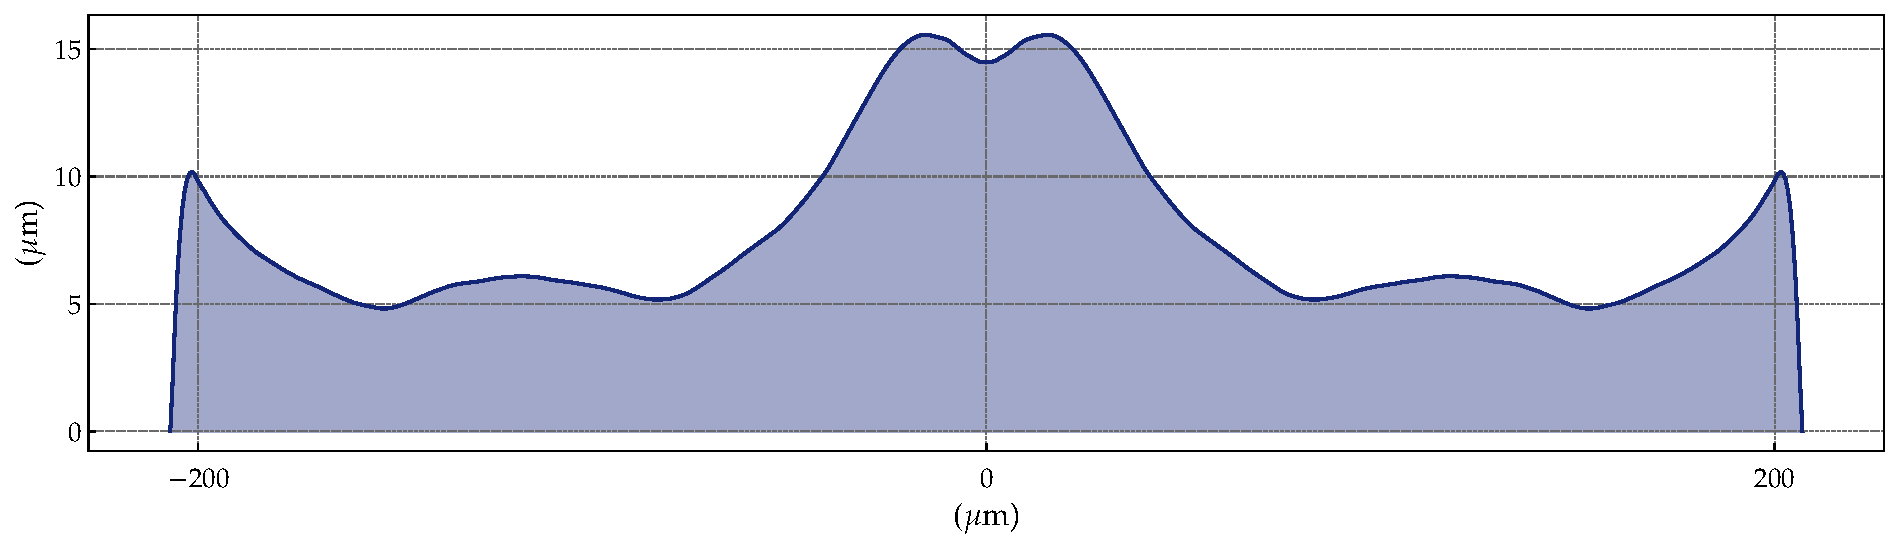
\includegraphics[width=0.6\linewidth]{figures/ch06/CDn_individual_8p0keV_n_10.0_lsp2p0mm_cpp10p0mm_phase_correction_plate_cut_2.pdf}}
        \caption[Diamond correction plate profile cut]{Profile cut of a diamond corrective plate for the lenses L01-L10 at 8~keV - cf. Fig.~\ref{fig:accumulated_profile_1}. The correction plate was calculated 10~mm downstream of the exit pupil of the CRL.}\label{fig:plate_profile}
\end{figure}

\begin{figure}[t]
        \centering
        {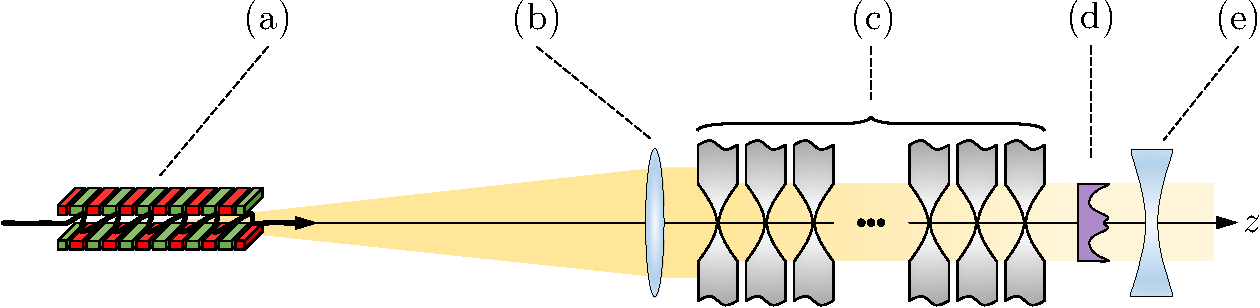
\includegraphics[width=0.6\linewidth]{figures/ch06/recovered_phase_corrected.pdf}}
        \caption[Schematic for residual thickness error calculation after phase correction]{Schematic for residual thickness error calculation after phase correction. (a) shows an arbitrary X-ray source. An (b) ideal parabolic phase element is placed downstream the radiation source to give the illumination a plane phase. The stacked X-ray lenses are placed immediately downstream. Any changes to the wave-field after (c) can be directly attributed to the model under study. The phase plate is placed in (d) to correct the accumulated phase errors. An (e) ideal parabolic phase element with a radius of curvature matching the developed quadratic term is then added and the residues (phase errors) can be extracted.}\label{fig:recovered_phase_corrected}
\end{figure}

\begin{figure}[t]
        \centering
        {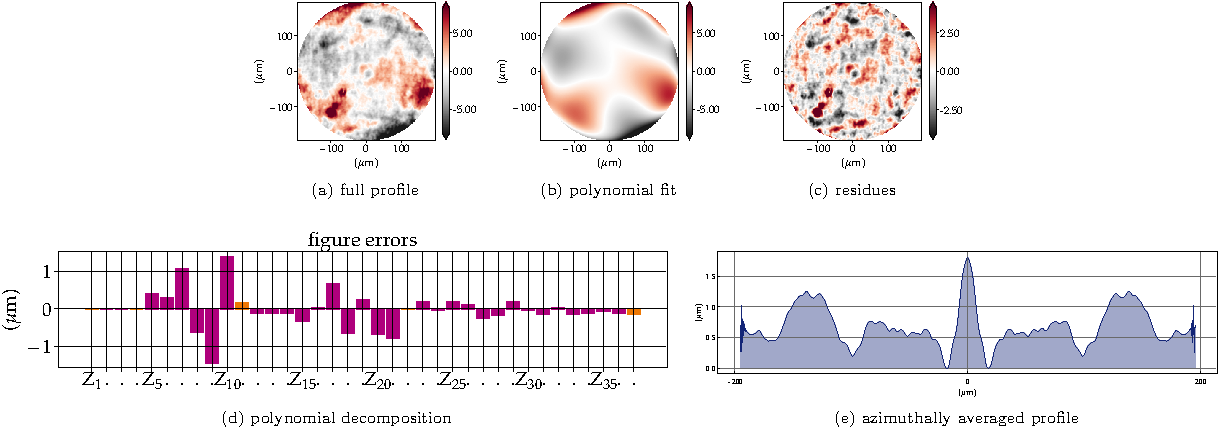
\includegraphics[width=1\linewidth]{figures/ch06/residual_profile.pdf}}
        \caption[Residual profile after phase correction]{Residual thickness error of the individually measured and artificially stacked lenses L01-L10 corrected with the diamond phase plate displayed in Fig.~\ref{fig:plate_profile}.}\label{fig:residual_profile}
\end{figure}

\begin{table}[h]
    \caption[Residual figure error profile r.m.s. value for L01-L10 and for the corrected system]{Residual figure error profile r.m.s. value for L01-L10 (Fig.~\ref{fig:accumulated_profile_1}) and for the corrected system (Fig.~\ref{fig:residual_profile}).}
    \centering
    \label{tab:corrected}\small
    \begin{tabular}{rccc}
    \hline \hline
    &\multicolumn{3}{c}{figure errors$^\dagger$ (r.m.s) $\mu$m}\\ \cline{2-4}
    &full profile & pol. fit   & residues \\ \hline
    L01-L10:      &4.84  &4.36  &2.18\\
    L01-L10 + PP: &3.27  &2.84  &1.63\\
    \hline \hline
    \multicolumn{4}{r}{\footnotesize{$^\dagger$ values given for $A_{\diameter}=400~\mu\text{m}$}}     
    \end{tabular}
\end{table}

\begin{table}[h]
    \caption[Strehl ratio for L01-L10 and for the corrected system]{Comparison of the Strehl ratio for aberrated system composed of L01-L10 and the corrected system as shown in Fig.~\ref{fig:Strehl_correction}.}\label{tab:Strehl_corrected}%\small
    \resizebox{\columnwidth}{!}{
    \centering
    \begin{tabular}{lrcccccc}\hline \hline
    &    &$\sigma_z$ ($\mu$m)     &$S_{\text{a}}$ (Eq.~\ref{eq:Strehl})  &$S_{\text{b}}$  (Eq.~\ref{eq:Marechal}) &$S_{\text{c}}$  (Eq.~\ref{eq:Mahajan}) &$S_{\text{ratio coh.}}$ &$S_{\text{ratio part.-coh.}}$ \\ \hline
    Fig.~\ref{fig:Strehl_correction} &L01-L10  &4.84  &0.067      &0.285 &0.393  &0.394         &0.409 \\
    &L01-L10 + PP                              &3.27  &0.503      &0.545 &0.608  &0.595         &0.671\\
    \hline \hline
    \end{tabular}
    }
\end{table}{}

%-------------------------------------------------------------------------
%-------------------------------------------------------------------------
\subsubsection*{Expected performance}
%-------------------------------------------------------------------------
%-------------------------------------------------------------------------

By reproducing the simulations from \S\ref{sec:coherent_sim}~-~\textit{\nameref{sec:coherent_sim}} and \S\ref{sec:partcoherent_sim}~-~\textit{\nameref{sec:partcoherent_sim}} to the corrected optical system as shown in Fig.~\ref{fig:optical_setups_corrected}, it is possible to evaluate the correction plate performance and predict its effect in a coherent- and partially-coherent X-ray beam. Figure~\ref{fig:CDn_corrected} summarises the simulations and can be directly compared to Fig.~\ref{fig:CDnS} as it
shows the beam profile at selected positions up- and downstream the focal plane for a (a) partially- and for a (b) coherent beam. The beam caustic is shown in Fig.~\ref{fig:CDn_corrected}(c), while the (d) phase and (e) amplitude of the PSF, as well as the (f) source image, are shown right next to it. A graphical representation of the Strehl ratio for the aberrated system and corrected system is shown in Fig.~\ref{fig:Strehl_correction} for the coherent and partially-coherent cases.

\begin{figure}[t]
        \centering
        {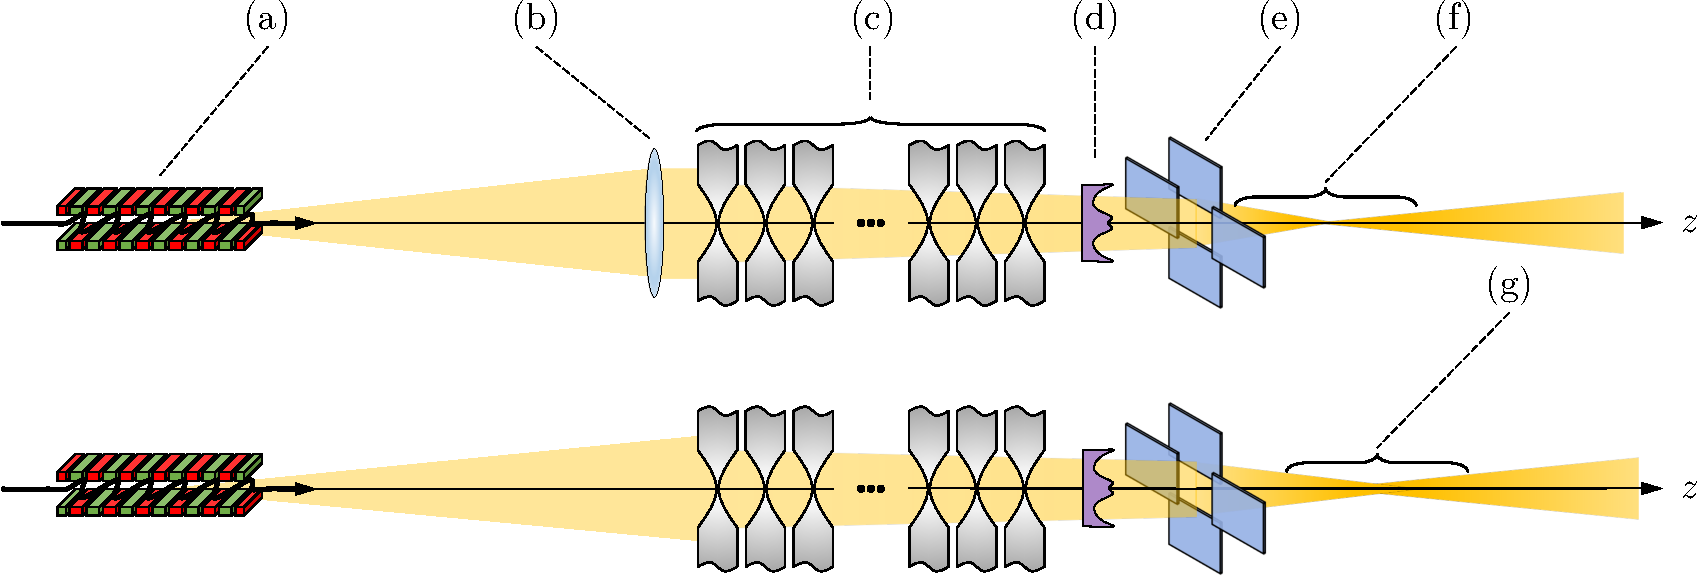
\includegraphics[width=0.8\linewidth]{figures/ch06/optical_setups_corrected.pdf}}
        \caption[Beamlines for coherent- and partially-coherent simulations]{\textbf{top row}: beamline used for  \S\ref{sec:coherent_sim}~-~\textit{\nameref{sec:coherent_sim}}. \textbf{bottom row}: beamline used for  \S\ref{sec:partcoherent_sim}~-~\textit{\nameref{sec:partcoherent_sim}}. (a) shows the X-ray source. An (b) ideal parabolic phase element is placed downstream the radiation source to give the illumination plane phase. This ideal element is only present for the fully-coherent simulations. The lenses being studied are shown in (c), which are followed by the (d) the correction plate. A set of (e) slits to ensure the same geometric aperture for all simulations. For the fully-coherent simulations, the beam-caustic range is shown in (f) and the PSF is calculated at the centre of it. For the partially-coherent simulations, the beam profile evolution along the optical axis is shown in (g) and the beam characteristics at the focal position are calculated at its centre. 
        }\label{fig:optical_setups_corrected}
\end{figure}

\begin{figure}[h]
        \centering
        {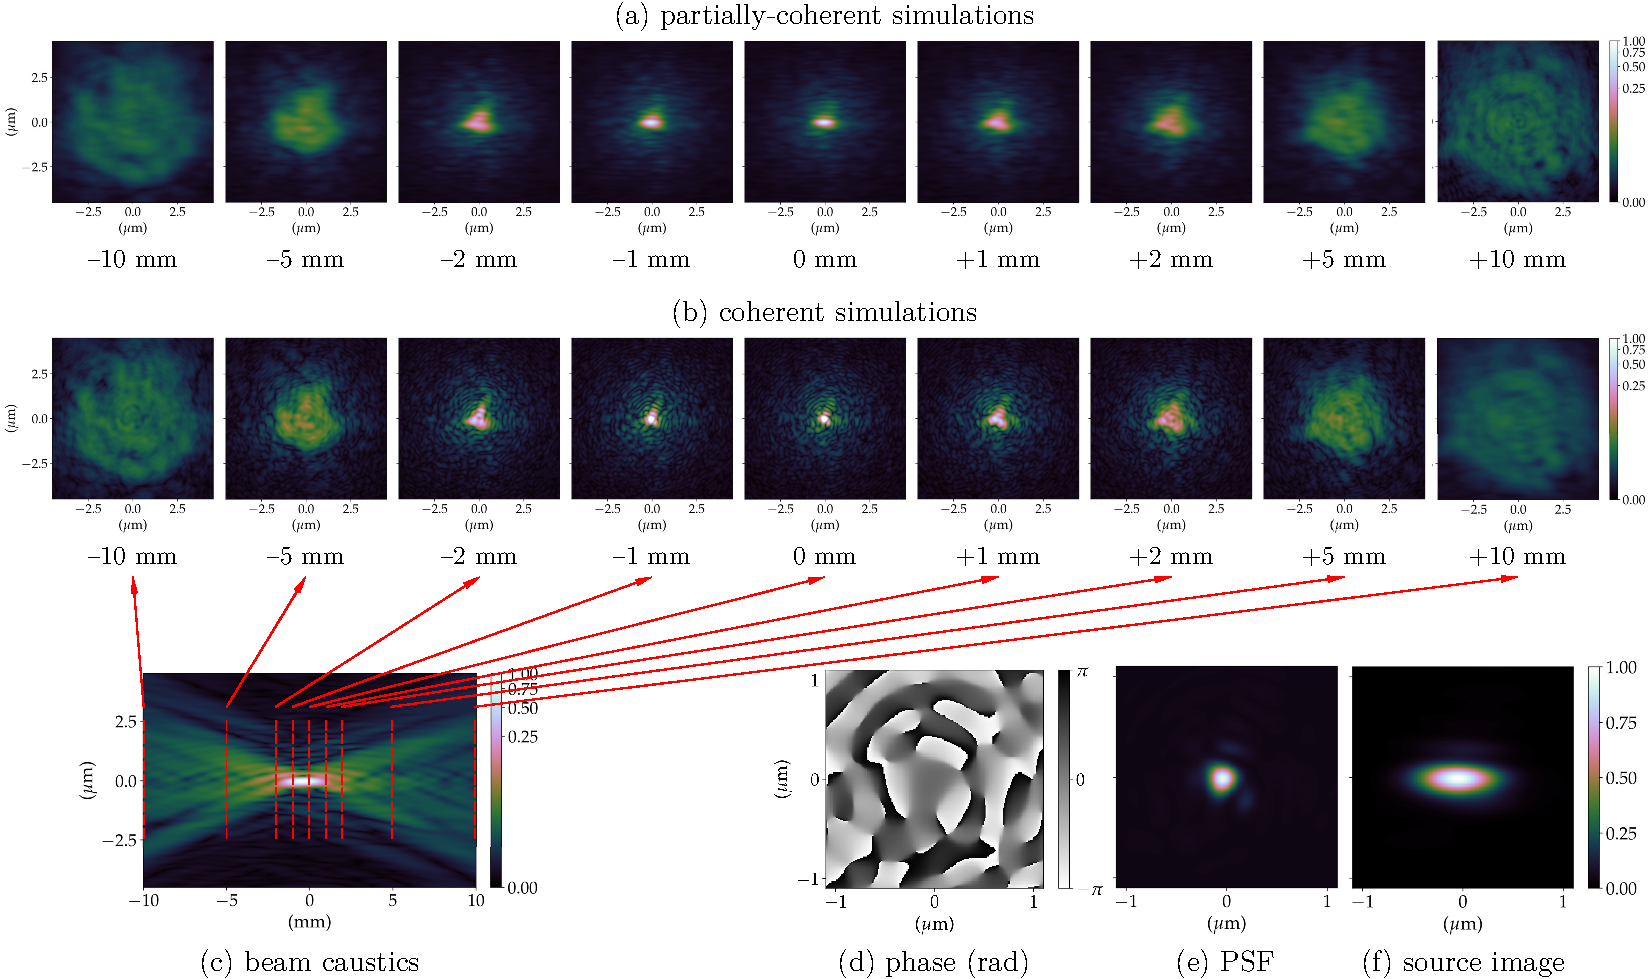
\includegraphics[width=0.99\linewidth]{figures/ch06/CDn_corrected.pdf}}
        \caption[Expected performance of the diamond phase corrector]{Expected performance of the diamond phase corrector. (a) partially-coherent simulations show the beam profile up- and downstream the focal position averaging 10$^{4}$ wavefronts to simulate the radiation emitted by an undulator; (b) the coherent simulations show the beam profile of a plane wavefront being focused; (c) beam propagation near the focal position (beam caustics) for a fully coherent beam (horizontal cut around $y=0$); (d) phase and (e) intensity of the PSF calculated focusing a plane-wavefront; (f) demagnified image of the undulator photon-source (extended source). The phase-plate was designed in diamond and a cut is shown in Fig.~\ref{fig:recovered_phase_corrected}. The residual error profile after the correction is shown in Fig.~\ref{fig:plate_profile}.}\label{fig:CDn_corrected}
\end{figure}

\begin{figure}[h]
        \centering
        {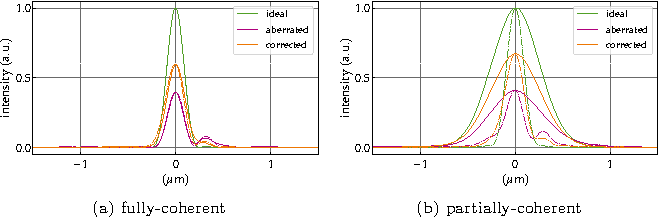
\includegraphics[width=0.7\linewidth]{figures/ch06/Strehl_correction.pdf}}
        \caption[Strehl ratio for the corrected system]{Visual representation of the Strehl ratio for the aberrated and corrected optical system. Coherent simulations are shown in (a) and partially-coherent simulations in (b) at 8~keV.}\label{fig:Strehl_correction}
\end{figure}

%-------------------------------------------------------------------------
%-------------------------------------------------------------------------
\subsubsection*{Tolerancing\footnote{This section came to be after some discussions with Andreas Schropp and Frank Seiboth (DESY, Germany) on the phase plate sensitivity to the alignment precision.}}
%-------------------------------------------------------------------------
%-------------------------------------------------------------------------

The expected performance of the correction plate shown in Figs.~\ref{fig:CDn_corrected} and \ref{fig:Strehl_correction} and compiled in the Tables~\ref{tab:corrected} and \ref{tab:Strehl_corrected} always assumes that the phase plate is perfectly centred in respect to the optical axis, at the designed distance $\Delta_{z_\text{pp}}$ from the CRL and that it presents no tilt in relation to the optical axis. However, when mounting the phase-plate in a real experimental setup, these are very difficult to reproduce. To understand and establish the precision to which the alignment has to be done, a series of scans is presented in Fig.~\ref{fig:tolerancing}, which shows the simulations of a (a) longitudinal, a (b) transverse and an angular scan of the phase plate around its nominal (designed) position. The transverse alignment is clearly very important. The longitudinal alignment is, to a lesser extent, also important. The plate shows a relative insensitivity to angular misalignments. Although Fig.~\ref{fig:tolerancing} shows only coherent simulations, it is believed that the results can be applied to a moderately partially-coherent X-ray beam without great loss.

\begin{figure}[h]
        \centering
        {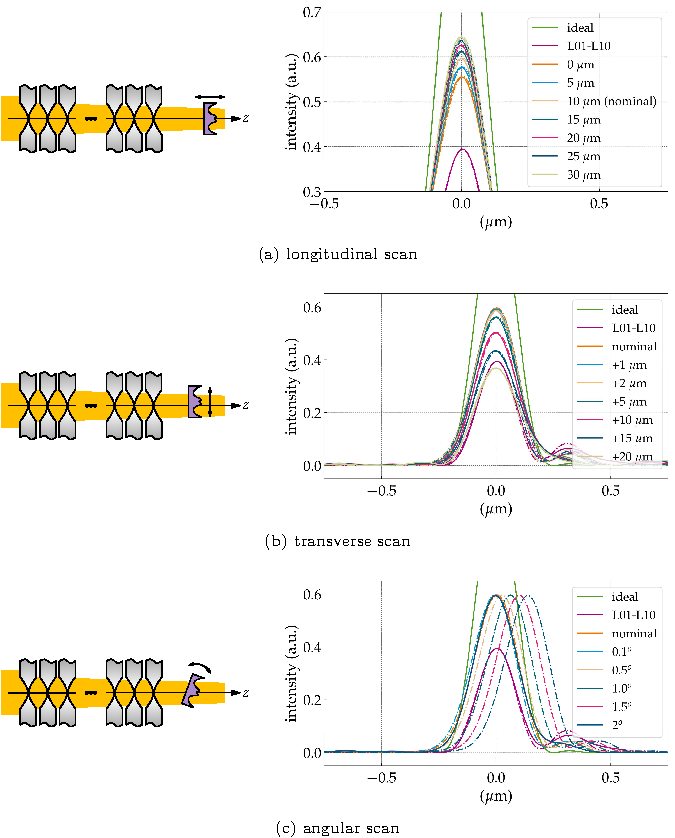
\includegraphics[width=0.7\linewidth]{figures/ch06/sensitivity_test.pdf}}
        \caption[Alignment sensitivity scan for the corrected system]{Study of the precision requirements on longitudinal, transverse and angular alignment of the phase plate based on the optimisation of the Strehl ratio for a fully-coherent beam.}\label{fig:tolerancing}
\end{figure}

\clearpage
%-------------------------------------------------------------------------
%-------------------------------------------------------------------------
\section{Prototype}\label{sec:prototype}
%-------------------------------------------------------------------------
%-------------------------------------------------------------------------

A series of phase plates designed to correct the accumulated figure error of 10 Be lenses (L01-L10) was commissioned based on the profile shown in Fig.~\ref{fig:plate_profile}, which was calculated to be placed 10~mm downstream the last lens of the stack and to correct the errors at 8~keV. The plates were ablated from diamond (HPHT IIb) by a femtosecond laser (515~nm, 3~W, 60~kHz, 200~fs) by a third-party company. The refractive phase plates produced by such technique have a surface roughness of $\sim$700~nm, but the company offers polishing, which lowers the surface roughness down to $\sim$100~nm, at the expense of removing some high-spatial frequency features of the correctors, but it is possible to account for the uneven material removal during polishing on the design of the phase plate\footnote{At the time of this writing this has not yet been tested.} [\cite{Antipov2020}]. Regardless of the surface finishing, a high shape fidelity to the profile in Fig.~\ref{fig:plate_profile} is expected from the prototypes. Lastly, to facilitate the use of the phase correctors, it was requested that the phase plates come in frames compatible with those used for X-ray lenses - see Fig.~\ref{fig:potpourri}. The phase-plate should be precisely centred in the $\diameter=12$~mm aluminium-bronze disk, so it can be easily installed in the lens housing minimising the performance degradation from misalignments shown in Fig.~\ref{fig:tolerancing}.

\begin{figure}[t]
        \centering
        {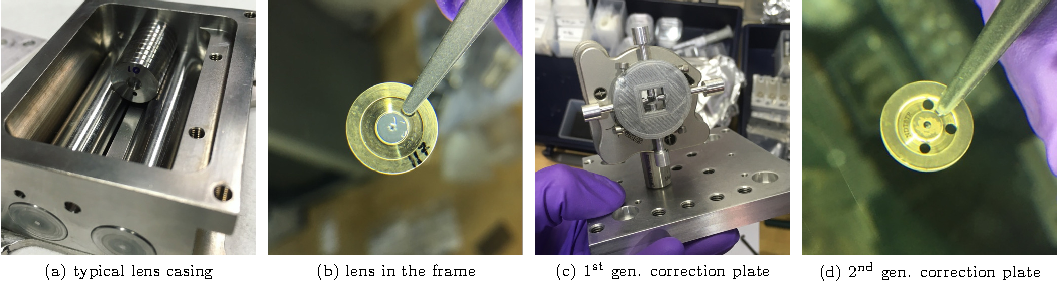
\includegraphics[width=1\linewidth]{figures/ch06/ppr.pdf}}
        \caption[Lens casing, frame and correction plates]{Typical lens casing, lens frame and both generation of correction plates. }\label{fig:potpourri}
\end{figure}
%-------------------------------------------------------------------------
%-------------------------------------------------------------------------
\subsection{Early tests on an X-ray beam}\label{sec:prototype_testing}
%-------------------------------------------------------------------------
%-------------------------------------------------------------------------

So far, only two generations of correction plates were produced - see Fig.~\ref{fig:potpourri}. The first generation of phase-plates was received and measured in Dec. 2019 with the XSVT technique described in \S\ref{sec:measuring}~-~\textit{\nameref{sec:measuring}}. This first iteration did not aim to produce useful plates, but it allowed to gain useful insights for the production of the second generation correctors, which was delivered in June 2020 - this time to be used for correction of optical imperfections in real CRLs. The phase-plates from the second generation design were chosen to demonstrate some of the preliminary results correcting optical imperfections in refractive lenses available at the ESRF.

The second generation of phase plates consisted of a set of three correction plates (PP01.v1 to PP01.v3) based on the design shown in Fig.~\ref{fig:plate_profile}. The difference among the three plates is the script used for laser ablation and the presence or not of surface post-processing. The v1 refers to an undisclosed laser polishing, while v2 and v3 have no post-processing. The PP01.v3 plate uses a different script for surface removal [\cite{Antipov2020}]. Figure~\ref{fig:pps} shows the retrieved profile using the XSVT technique and experimental setup described in \S\ref{sec:measuring}~-~\textit{\nameref{sec:measuring}}. The profiles are very similar among each other and no strong effect in the surface shape of the polished phase-plate can be observed with XSVT. For the phase-plate PP01.v2, the manufacturer provided visible light metrology (scanning confocal laser microscopy), which is shown in Fig.~\ref{fig:pp2_visible}. The surface roughness of the non-polished plate is evident in Fig.~\ref{fig:pp2_visible}(c). Figure~\ref{fig:metrology_comp} shows a profile cut of the retrieved thicknesses measured with XSVT and visible-light metrology against the designed profile, showing a initial good agreement for the central part of the phase plate and lesser agreement towards the edge of the geometric aperture.  

Once measured individually, the phase plates were added directly to the lens casing relying on the assumption that the phase-plates were perfectly centred within their frames and thus, would ideally be perfectly aligned to the lens stack - see Fig.~\ref{fig:potpourri}. The lens stack with the correction plate was then re-measured with the XSVT. For comparison, the lens stack without any correction was also measured under the very same conditions. The metrology is shown in Fig.~\ref{fig:alignment_xsvt} and summarised in Table~\ref{tab:corrected_xsvt}. It is evident that the correction plates are not centred within the lateral tolerance defined by Fig.~\ref{fig:tolerancing}(c)-(d) as no significant improvement in the residual profile can be seen.

\begin{table}[t]
    \caption[Residual figure error profile r.m.s. value for L01-L10 and for the corrected system]{Residual figure error profile r.m.s. value for L01-L10 (Fig.~\ref{fig:accumulated_profile_1}) and for the corrected system (Fig.~\ref{fig:residual_profile}).}
    \centering
    \label{tab:corrected_xsvt}\small
    \begin{tabular}{rccc}
    \hline \hline
    &\multicolumn{3}{c}{figure errors$^\dagger$ (r.m.s) $\mu$m}\\ \cline{2-4}
    &full profile & pol. fit   & residues \\ \hline
    stack 01:           &4.89  &4.73  &1.41\\
    stack 01 + PP01.v1: &3.03  &2.91  &1.66\\
    stack 01 + PP01.v2: &4.26  &3.95  &1.51\\
    stack 01 + PP01.v3: &3.44  &3.10  &1.44\\
    % stack 01 + PP02.v1: &4.86  &4.81  &1.78\\
    % stack 01 + PP02.v2: &4.09  &3.84  &1.33\\
    % stack 01 + PP02.v3: &3.59  &3.34  &1.21\\
    \hline \hline
    \multicolumn{4}{r}{\footnotesize{$^\dagger$ values given for $A_{\diameter}=320~\mu\text{m}$}}     
    \end{tabular}
\end{table}

To be able to test the correction effectiveness and performance, it was decided to mount a phase-plate outside the lens case so at least the transverse alignment could be done. The phase-plate chosen for these tests was the PP01.v2 due to its good agreement with he designed profile in Fig.~\ref{fig:plate_profile}. The simplest alignment of the phase plate is based on maximising the peak intensity at the image plane. This approach, however, could not be employed due to the saturation of the detector at the image plane even after a set of attenuators was used. Instead, the alignment of the phase-corrector was done trying to visually optimise, in terms of homogeneity, the far-field beam-profile several tens of millimetres downstream the focal plane. Once the best transverse position was found, a series of 2D images up- and downstream the optical axis was taken with the same 2D imaging detector used for the XSVT (pixel size of $\sim$0.63~$\mu$m). The beam caustics can be obtained from this series of images and it is shown in Fig.~\ref{fig:experimental_CDn_pp} for the aberrated and corrected system. Due to the saturation in the vicinity of the focal plane, a quantitative assessment of the improvement cannot be done, however, a clear qualitative improvement on the beam profile up- and downstream the focal plane is seen.


\clearpage

\begin{figure}[t]
        \centering
        {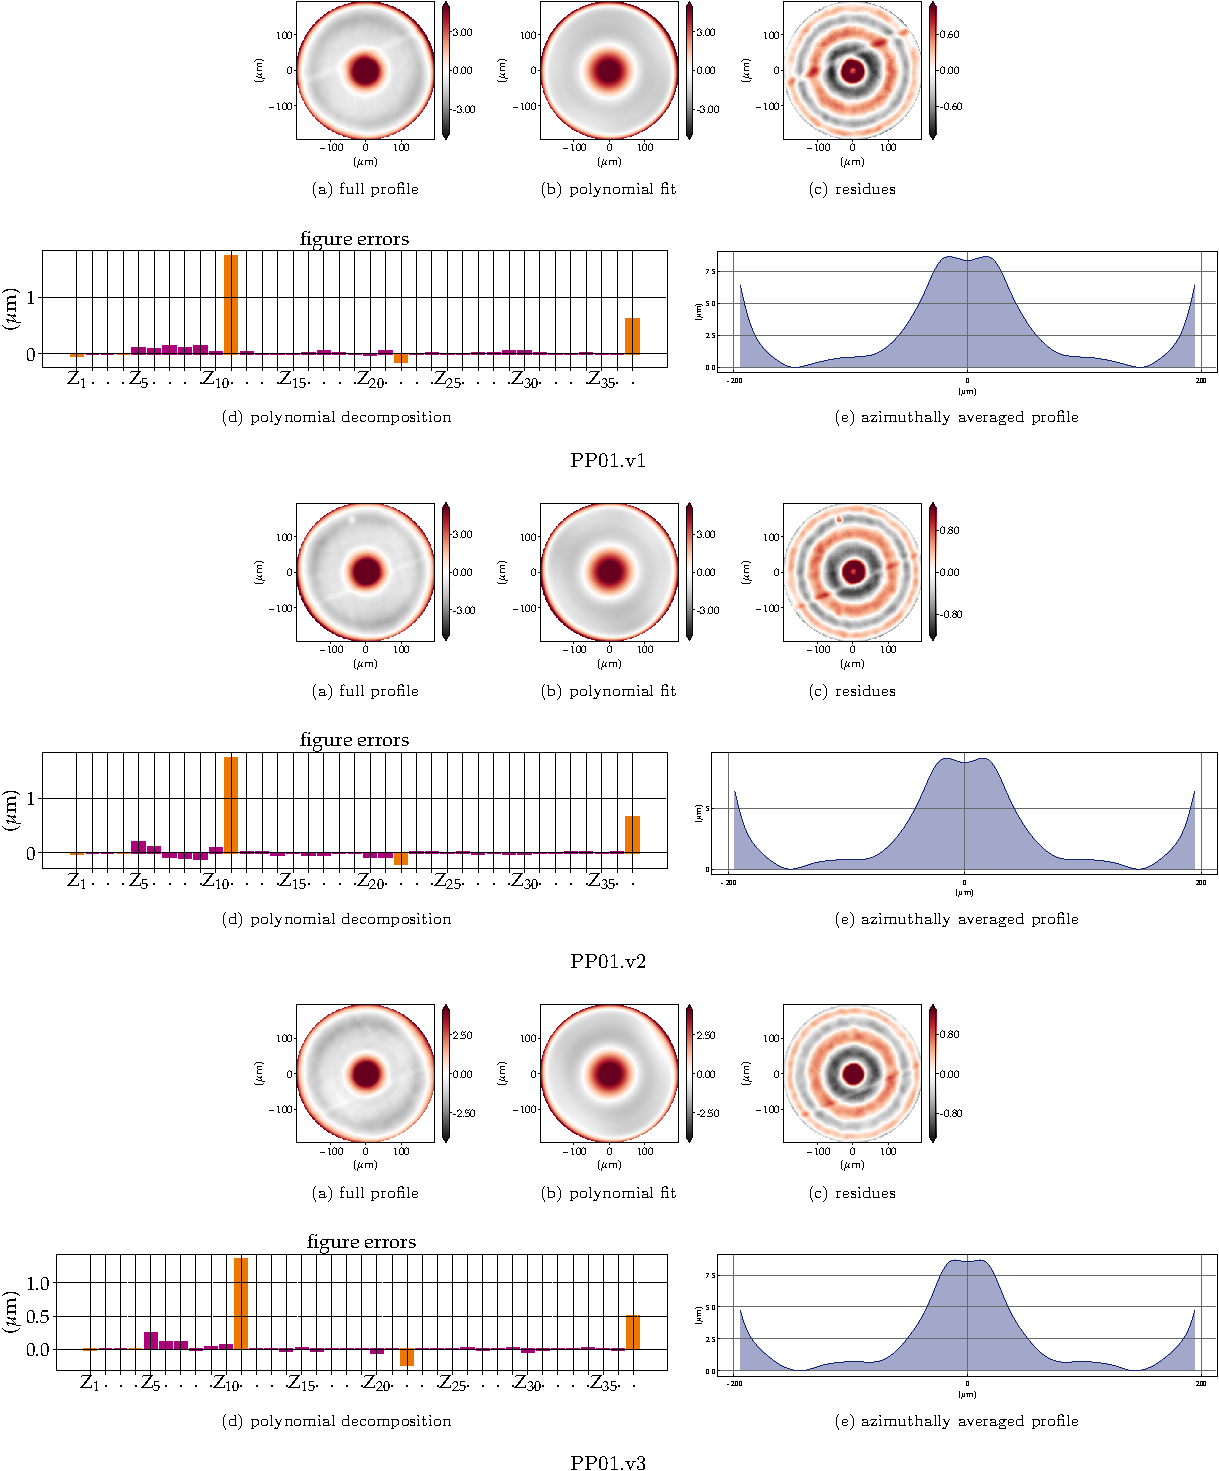
\includegraphics[width=1\linewidth]{figures/ch06/pps.pdf}}
        \caption[XSVT metrology of phase-plate PP01.v1-PP01.v3]{Phase-plate metrology using the XSVT as described in \S\ref{sec:measuring}~-~\textit{\nameref{sec:measuring}}.}\label{fig:pps}
\end{figure}

\begin{figure}[t]
        \centering
        {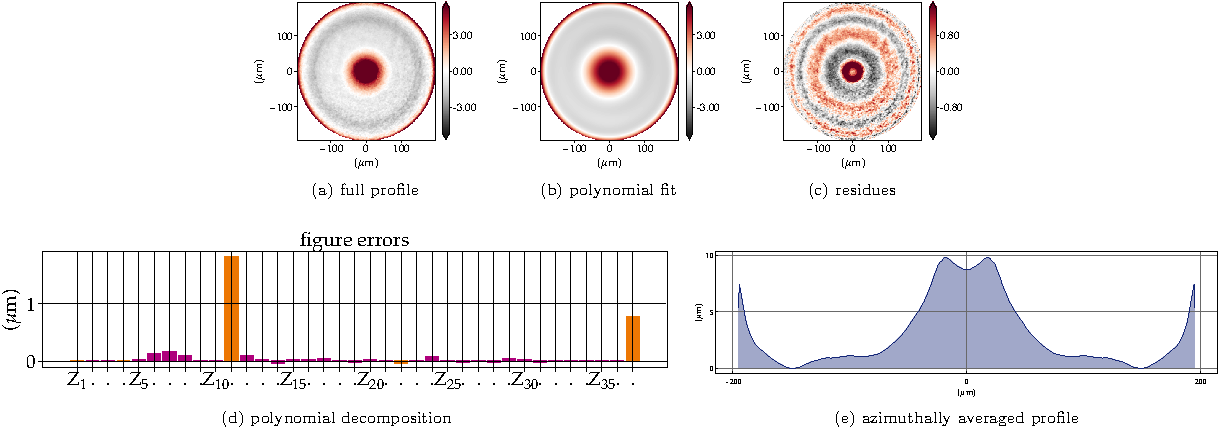
\includegraphics[width=1\linewidth]{figures/ch06/pp2_visible.pdf}}
        \caption[Scanning confocal laser microscopy of PP01.v2 phase-plate]{Scanning confocal laser microscopy of the PP01.v2 phase-plate provided by the manufacturer.}\label{fig:pp2_visible}
\end{figure}

\begin{figure}[t]
        \centering
        {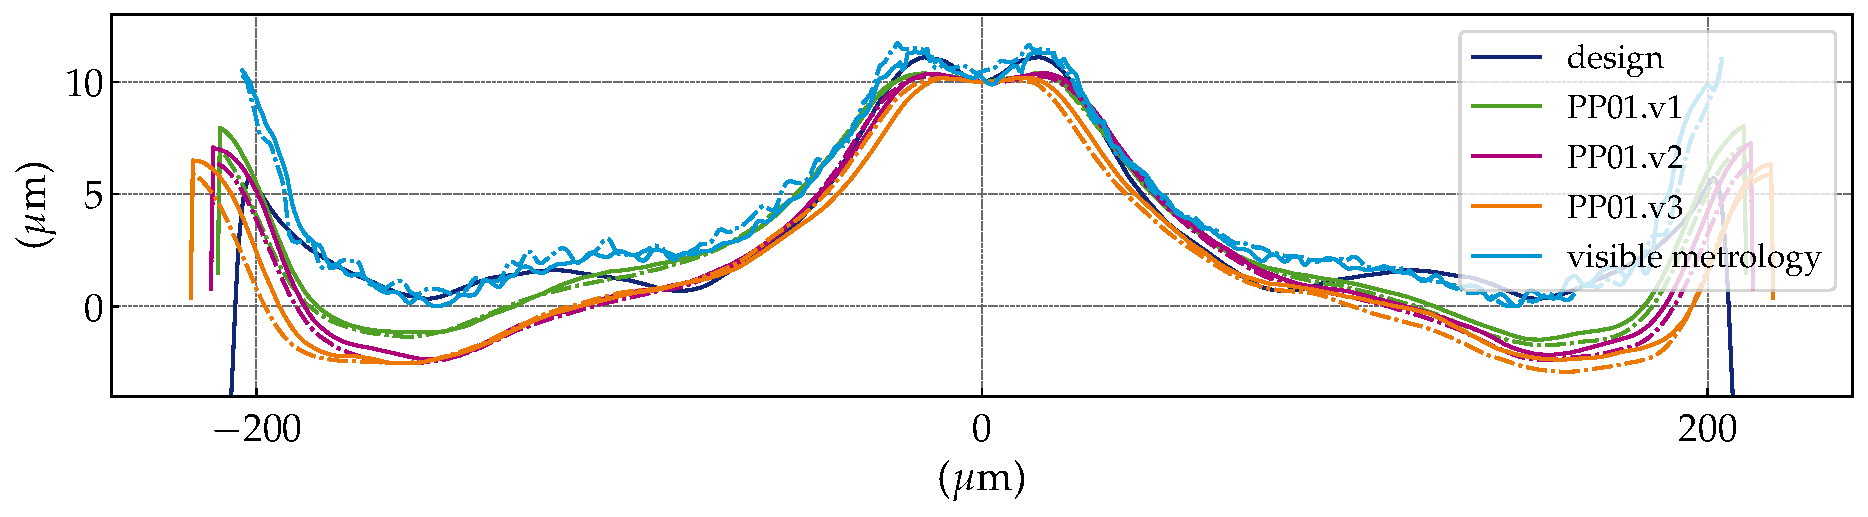
\includegraphics[width=0.7\linewidth]{figures/ch06/metrology_comp.pdf}}
        \caption[Profile cuts of the correction plates]{Profile cuts of the correction plates P01.v1-v3 measured with the XSVT metrology and from the P01.v2 plate measured with the visible-light metrology. }\label{fig:metrology_comp}
\end{figure}

\begin{figure}[t]
        \centering
        {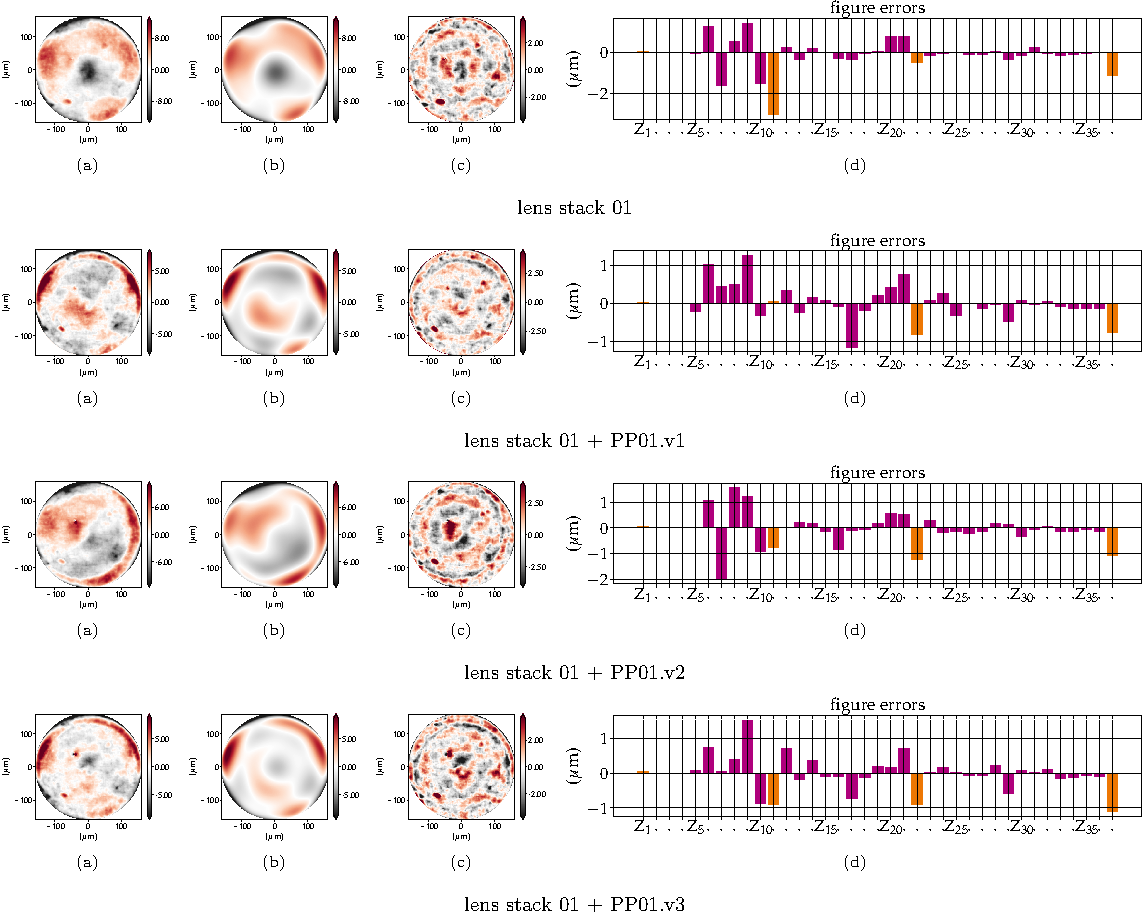
\includegraphics[width=1.0\linewidth]{figures/ch06/alignment_xsvt.pdf}}
        \caption[Residual thickness after installation of the correction plates PP01.v1-v3]{\textbf{top row}: thickness error of lens stack 01. \textbf{centre-top} to \textbf{bottom row}: residual thickness after installation of the correction plates PP01.v1, PP01.v2 and PP01.v3 respectively.}\label{fig:alignment_xsvt}
\end{figure}

\clearpage

\begin{figure}[t]
        \centering
        {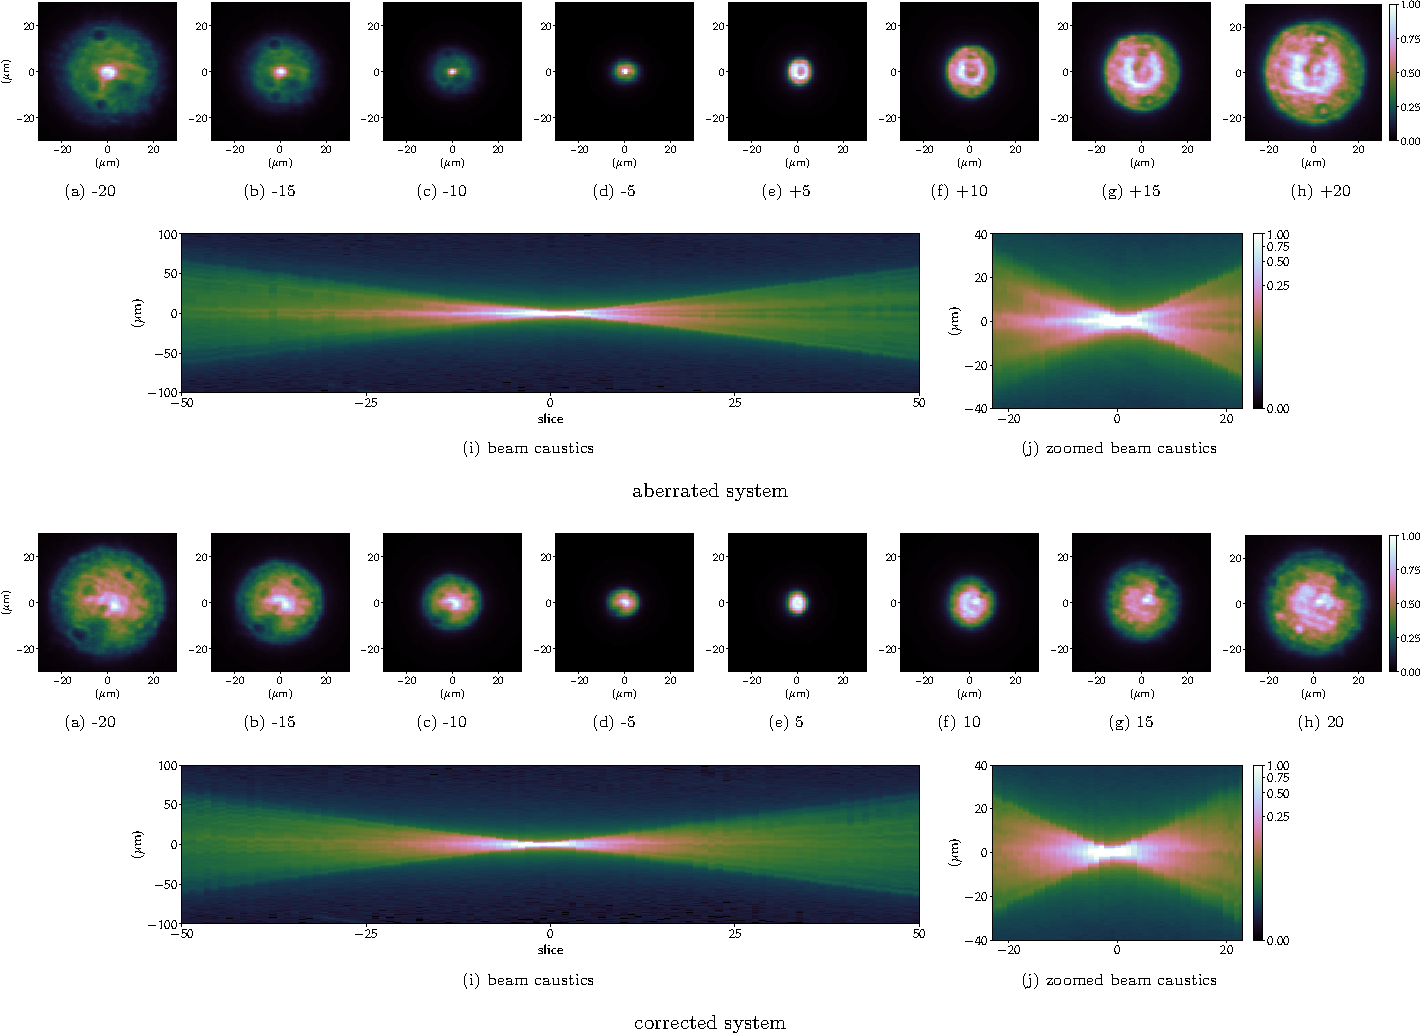
\includegraphics[width=1.0\linewidth]{figures/ch06/experimental_CDn_pp.pdf}}
        \caption[Experimental beam caustics for the aberrated and corrected systems]{Experimental beam caustics taken at 10.6~keV for the aberrated and corrected system.}\label{fig:experimental_CDn_pp}
\end{figure}
%-------------------------------------------------------------------------
%-------------------------------------------------------------------------
\section{Discussion}\label{sec:corrective_optics_discussion}
%-------------------------------------------------------------------------
%-------------------------------------------------------------------------

\subsection{Design and expected performance}

The concept and design of optical correction for the aberrated system are quite simple and can be represented by the Eq.~\ref{eq:phase_plate}. Although current micro- and nano-manufacturing techniques can reproduce such intricate profiles, its alignment on a beamline can be cumbersome and render the correction plate impractical. A successful compromise for 2D focusing CRLs is the adoption of a radially symmetric correction plate described by Eq.~\ref{eq:phase_plate_r} - these have been demonstrated to work by other groups [\cite{Seiboth2017,Seiboth2018,Seiboth2020,Dhamgaye2020}]. 

Using the approach guided by Eq.~\ref{eq:phase_plate_r}, a design to compensate for the accumulated errors from lenses L01-L10 (see  Fig.~\ref{fig:accumulated_profile_1}) was calculated and it is shown in Fig.~\ref{fig:plate_profile}. Placing this ideal diamond phase-plate on the simulations and extracting the residual profile allows gaining some insight into the expected performance of the corrected system. Although most, if not all spherical aberration was removed, there is still a high content on non-symmetric aberrations as shown in Figure~\ref{fig:residual_profile}(d), which will still degrade the beam focusing quality, but to a lesser extent. Figure~\ref{fig:residual_profile}(e) shows a (much reduced) residual profile, which indicates that the correction plate should be calculation over a few iterations until the azimuthally averaged profile goes below what is currently possible to be manufactured. Table~\ref{tab:corrected} shows that the overall figure error r.m.s. value over the exit pupil is reduced to $\sim$68\% of the L01-L10 figure error. The low-frequencies are more affected, being reduced to 65\% its original value. The high frequencies are reduced to 75\% of the value before the correction. This reduction in the figure errors is accompanied by an increase in the Strehl ratio as evidenced by Table~\ref{tab:Strehl_corrected} and Fig.~\ref{fig:Strehl_correction}. The improvement of the Strehl ratio for the coherent case differs from the one for the partially-coherent case. Figure~\ref{fig:Strehl} already showed a very small difference between both cases, but it was deemed to be insignificant. This difference shows the necessity of further studying the impact of the optical correction for moderate- and low-coherence systems.

The expected improvements brought by the optical correction also apply to the beam up- and down-stream the image plane as the several cuts along the beam caustics in Fig.~\ref{fig:CDn_corrected} show. The elongated tail before the image plane and the doughnut shape from Fig.~\ref{fig:CDnS} are no longer present, however, at the image plane vicinity, satellite structures are seen around the main lobe. The image plane is greatly improved for both the fully- and partially-coherent simulations with great suppression of the side lobes, showing some similarities with the beam performance predicted in Fig.~\ref{fig:simulations_HF}. In fact, the better the correction plate is, the closer the system will behave as in Fig.~\ref{fig:simulations_HF}, a result of the high-frequency profile shown in Fig.~\ref{fig:CDnHF}. The performance of very well corrected systems will be limited by the high-frequency content, which does not significantly changes the main-lobe, but significantly increases the background around it, as shown in Fig.~\ref{fig:hf_strehl_scan}.

It is important to point out that the expected performance and all previously improvements are only obtained for the perfectly aligned phase-plate. Tolerance simulations were done to narrow down the most critical degrees of freedom when aligning the phase-plate in respect to the CRL to be corrected. The longitudinal scan is a useful tool when operating the phase plate outside the design energy. Figure~\ref{fig:tolerancing}(a)-(b) shows that a longitudinal scan of a phase-plate operating at its designed energy. Bringing the plate upstream of the nominal position $\Delta_{z_\text{pp}}$ degrades its performance, but going downstream moderately improves it. This is probably due to the higher absorption towards the edge of the plate and a smaller footprint of the beam. The transverse alignment is by far the most sensitive degree of freedom and a moderate misalignment may compromise the correction, bringing the Strehl ratio to the same value the aberrated system originally had. Figure~\ref{fig:tolerancing}(c)-(d) reinforces what has been observed by other groups [\cite[Fig.~5.12]{Seiboth2016b}]. Finally, in terms of the Strehl ratio, the phase-plate is not too much influenced by the angular alignment, provided it is kept reasonably small. A tilt is introduced to the system, which laterally shifts the focused beam, but its intensity remains largely unchanged.

\subsection{Early phase plate tests on an X-ray beam}

The early tests with the second generation of phase-plate are encouraging and help delineate strategies for further development of phase correctors to be used with the CRLs. Three phase plates were produced trying to replicate the shape in Fig.~\ref{fig:plate_profile} with differences in the scripts used for engraving the diamond slab and with post polishing or not. Figures~\ref{fig:pps} and \ref{fig:pp2_visible} show a very similar profile for all three plates where the low-frequencies are well represented, but the residues from the polynomial fit show a clear limitation of XSVT in showing the difference between a polished and non-polished plate. Although the effects of polishing are noticeable in the far-field (presence of small-angle scattering and speckle), XSVT cannot show the surface roughness as visible-light metrology does - Fig.~\ref{fig:pp2_visible}. This makes the case for using complementary metrology methods for a complete characterisation of the phase-plates. When overlapping the profile cuts, as in Fig.~\ref{fig:metrology_comp}, the difference in the profiles becomes more evident. Visible light metrology and designed plate have a more similar profile, while the data collected with XSVT show lower height values towards the edges of the phase-plate. The differences may come from the processing of the phase-gradients from the XSVT, small inaccuracies when measuring the distances in the experimental setup or a difference between the tabled index of refraction/density and the real index of refraction from the plate - something similar has been speculated in [\cite[\textit{§3.2}]{Seiboth2020}] for justifying differences between design and measured phase-plates produced using IP-S resist, a much less studied material than diamond. 

One of the key aspects of the commissioned phase-plates is that they come perfectly centred in a frame compatible to the ones used for encasing X-ray lenses - Fig.~\ref{fig:potpourri}(b) and (c), which is done to circumvent the degradation in performance from the lateral misalignment in Fig.~\ref{fig:tolerancing}(c)-(d). Unfortunately, the phase plates of the current generation do not yet meet such requirements as the metrology of the CRL with the correction plates suggests - see Fig.~\ref{fig:alignment_xsvt}; improvements in the centring of the phase plates are expected from the partner company, but are also separately under way within the X-ray optics group at the ESRF. 

Aligning the phase-plate to the CRL also revealed a very important aspect: the lack of an internal protocol for alignment. Ideally, one would scan the phase-plate transversely at each position of the scan, the residual wavefront would be calculated and the minimisation of figure errors would be sought. This approach is impractical for the XSVT due to the data acquisition and processing time, not to mention the very large data-set it would generate. This highlights the necessity to re-implement speckle-tracking based on only two images (XST)\footnote{Refer to \S\ref{sec:foundation}~-~\textit{\nameref{sec:foundation}} in \S\ref{sec:measuring}~-~\textit{\nameref{sec:measuring}}.} for a fast evaluation of the figure errors at the expense of a lower spatial resolution. This technique was less frequently used within the X-ray Optics Group due to the many advantages of XSVT [\cite{Berujon2020}], but there is a necessity to use XST for a faster characterisation.

Trying to align the phase-plate by maximising the peak intensity was the next obvious step. However, these particular experiments took place at the ID06 beamline after the ESRF-EBS upgrade, an undulator beamline that naturally has a very high photon flux at the harmonics when compared to the typical emission of bending magnets\footnote{Refer to \S\ref{sec:sources}~-~\textit{\nameref{sec:sources}}.}. This increase in photon flux is welcome for the metrology but causes the imaging detector to saturate at the image plane even after attenuators were placed in the beam. As an alternative to the optimisation of the peak intensity, the qualitative improvement of the beam profile downstream the focal plane was done. The phase plate was scanned transversely while the far-field was registered. The final position of the phase plate was where the beam was more homogeneous and the doughnut shape less evident. The drawing of general guidelines for the alignment of the phase-plates and metrics to evaluate it are the topic of future work\footnote{With the resumption of the ESRF user service mode, more access to beamtime is expected. The ESRF reopened to the public on the 25$^\text{th}$ of August 2020, despite the COVID-19 pandemic [\cite{Cho2020}].}.

The beam caustics and profiles shown in Fig.~\ref{fig:experimental_CDn_pp} for the aberrated beam confirm the results from the modelling presented in the chapter~\ref{sec:effect_optical_imperfections}~-~\textit{\nameref{sec:effect_optical_imperfections}} and published in [\cite{Celestre2020}]. The presence of the tail upstream of the focal plane and the doughnut shape downstream are clearly present. A direct comparison with the simulations is not possible due to the limited caustic step and detector pixel size, but the main elements and trends are present. Once the phase-plate is inserted and aligned, an improvement in the beam profile homogeneity is seen, although quantification is not possible, due to the saturation of the detector. The central tail is reduced, although still present upstream the image plane. More remarkable is the suppression of the doughnut shape. The performance of the correction plate is better near the image plane, but that could be from the low spatial resolution of the detector. 

\begin{figure}[t]
    \centering
    {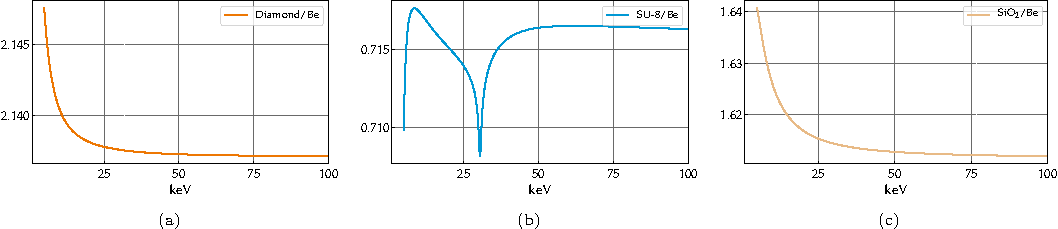
\includegraphics[width=1\linewidth]{figures/ch03/n_plate.pdf}}
    \caption[Index of refraction ratio for common phase plate materials]{(a) diamond, (b) SU-8 and (c) fused silica (SiO$_2$) refraction index decrement ratio against beryllium. Figures obtained using the \textit{xraylib} library [\cite{Brunetti2004, Schoonjans2011}].}
    \label{fig:delta_correction_plate}
\end{figure}

The experiments were conducted at 10.6~keV, while the design of the phase-plate was optimised for 8~keV. As mentioned previously, the correction plates can be used outside the designed energy if they were calculated for a modest number of lenses by shifting them along the optical axis as described by [\cite[\textit{\S6}]{Seiboth2018}]. Figure~\ref{fig:delta_correction_plate} shows the ratio of the index of refraction decrement and the $\delta$ of beryllium, which confirms an almost negligible variation over such a small energy difference. Figure~\ref{fig:delta_correction_plate} reinforces the conclusions in [\cite[\textit{\S6}]{Seiboth2018}] for commonly used phase plate materials.

The correction performance is, at the moment, far from the expected simulated performance or the reported performance from other groups [\cite{Seiboth2017,Seiboth2018,Seiboth2020,Dhamgaye2020}]. These are the performance of second-generation phase plates and with beamtime availability. Addressing the aforementioned issues with alignment, wavefront-sensing and protocols for evaluating the performance of the phase-plates, improvements in the design and fabrication of phase plates are expected.  $\blacksquare$

\addcontentsline{toc}{section}{References}
\printbibliography[heading=subbibliography]
\end{refsection}
